%%%%%%%%%%%%%%%%%%%%%%%%%%%%%%%%%%%%%%%%%%%%%%%%%%%%%%%%%%
%%
%% MARK: Title
%%
%%%%%%%%%%%%%%%%%%%%%%%%%%%%%%%%%%%%%%%%%%%%%%%%%%%%%%%%%%

\chapter*{\S B19. Differential of a Lie-Group Valued Function}
\setcounter{footnote}{0}

%%%%%%%%%%%%%%%%%%%%%%%%%%%%%%%%%%%%%%%%%%%%%%%%%%%%%%%%%%
%%
%% MARK: Abstract
%%
%%%%%%%%%%%%%%%%%%%%%%%%%%%%%%%%%%%%%%%%%%%%%%%%%%%%%%%%%%

\begin{abstract}
  In this note we give a meaning to the differential of a smooth function defined on a diffeological space,
  with values in a Lie group.
\end{abstract}

%%%%%%%%%%%%%%%%%%%%%%%%%%%%%%%%%%%%%%%%%%%%%%%%%%%%%%%%%%
%%
%% MARK: The General Question
%%
%%%%%%%%%%%%%%%%%%%%%%%%%%%%%%%%%%%%%%%%%%%%%%%%%%%%%%%%%%

\section{The general question}

This question was raised by Cheyne Miller,%
\footnote{Private email exchange of February 27, 2016.}
as a byproduct of his reflection on the differential of the holonomy function,
in the case of a general fiber bundle, or a more general situation.
I am sure he will not object to my sharing my reflection on his question in these notes.

Precisely,
a part of his question translates into:

\uline{Question} (Cheyne Miller) {\itshape Let $h : X \to G$ be a smooth function defined on a general diffeological space,
with values in an ordinary Lie group. What would be the meaning of $dh$?}

When $G$ is the abelian group $(\RR,+)$, we know the answer:
$$
  dh = h^*(dt),
$$
where $dt$ is the standard $1$-form on $\RR$.
More recently we have seen,
in the previous note ``Differential of Holonomy for Torus Bundles'',
that we can define a ``differential'' $d_{Torus} h$ by:
$$
  d_{Torus} h = h^*(\theta),
$$
where $\theta$ is the standard $1$-form on the (possibly irrational) torus $\Torus = \RR/\Gamma$,
the pushforward of $dt$ by the projection $\pi : \RR \to \Torus$.
In other words,
satisfying $\pi^*(\theta) = dt$.

We remark that,
in these two cases,
the differential of the function is the pullback of some fundamental form defined on the group $\RR$ or $\Torus$.
This observation will guide us in defining more generally the differential of a function with values in any Lie group.

%%%%%%%%%%%%%%%%%%%%%%%%%%%%%%%%%%%%%%%%%%%%%%%%%%%%%%%%%%
%%
%% MARK: The Maurer-Cartan Form
%%
%%%%%%%%%%%%%%%%%%%%%%%%%%%%%%%%%%%%%%%%%%%%%%%%%%%%%%%%%%

\section{The Maurer-Cartan form}

There is a canonical $1$-form defined on any Lie group $G$,
with values in the tangent space $\cG = \Tgt_\Id(G)$,
namely,
the Maurer-Cartan form $\Theta \in \DForms^1(G,\cG)$.
With the ordinary notations of differential calculus on a Lie group,
let $g \in G$,
let $\Lm(g)$ be left-multiplication by $g$,
that is,
$\Lm(g)(g') = gg'$.
Let $\delta g \in T_g G$
be any tangent vector at the point $g$,
then the Maurer-Cartan form $\Theta$ is defined by%
\footnote{The notation $\Der(f)(x)$ denotes the tangent linear map of $f$ at the point $x$.}
$$
  \Theta_g(\delta g) = [\Der(\Lm(g))(\Id)]^{-1}(\delta g).
$$
This Maurer-Cartan form is left-invariant,
that is,
$\Lm(k)^*(\Theta) = \Theta$ for all $k \in G$.
There is also an analogous right-invariant Maurer-Cartan form,
obtained by replacing $\L(g)$ with $R(g)$ in the definition above.
The choice depends on our needs or preferences.

Note that the Maurer-Cartan form has a diffeology-compliant definition.
Let $P : r \mapsto g_r$ be an $n$-plot of $G$,
let $v \in \RR^n$,
then:
$$
  \Theta(P)_r(v) = \Der\!\left(s \mapsto g_r^{-1} g_{r+s}\right)\!(s=0)(v).
$$

%%%%%%%%%%%%%%%%%%%%%%%%%%%%%%%%%%%%%%%%%%%%%%%%%%%%%%%%%%
%%
%% MARK: The Definition of the Differential
%%
%%%%%%%%%%%%%%%%%%%%%%%%%%%%%%%%%%%%%%%%%%%%%%%%%%%%%%%%%%

\section{The definition of the differential}

Now we have the tools to define the differential of the smooth function $h : X \to G$.
I suggest the following:

\begin{Article}{Definition.}{\itshape
  Let $X$ be a diffeological space,
  let $G$ be an ordinary Lie group,
  and let $h : X \to G$ be a smooth function.
  We define the {\em differential} of $h$ as the pullback by $h$ of the Maurer-Cartan form,
  and denote
  $$
    d_G h = h^*(\Theta),
    \qquad
    d_G h \in \DForms^1(X,\cG).
  $$
}
\end{Article}

This is a well-defined diffeological $1$-form with values in a vector space,
and it corresponds exactly to what we did in the particular abelian cases of $\RR$ or $\Torus$.
In those cases the Maurer-Cartan form is just the identity.

Now,
why is this a good replacement for the differential in the general case?
If $X$ is a manifold,
we have for all $x \in X$ and $\delta x \in \Tgt_x(X)$:
$$
  dh_x(\delta x) \in \Tgt_{h(x)}(G),
$$
where $dh_x$,
also denoted by $\Der(h)(x)$,
is the tangent linear map of $h$ at the point $x$.
The Maurer-Cartan form is precisely the tool for trivializing the tangent bundle.
The map $(g,v) \mapsto (g,\Theta_g(v))$ is the canonical isomorphism from $TG$ to $G \times \cG$.
Therefore $\Theta_{h(x)}(dh_x(\delta x))$ is the image of $\delta x$ by $dh_x$ after trivialization.

On the other hand,
$\Theta_{h(x)}(dh_x(\delta x))$ is,
by definition,
$h^*(\Theta)_x(\delta x)$.
Therefore,
the definition given above, $d_G h = h^*(\Theta)$, seems to be a good replacement,
in diffeology,
for the differential of a Lie-group-valued smooth function.

Note that in the $1$-dimensional case $G = \RR$ or $\Torus$ the differential $d_G h$ is closed
(because $2$-forms on $1$-dimensional spaces vanish),
which is no longer true in the general case.
Indeed,
$d[d_G h] = h^*(d\Theta) \in \DForms^2(X,\cG)$.
The differential $d_G$ is a replacement for the tangent linear map,
not for the differential operator of exterior calculus.
But this is what is useful in mathematical physics when one deals with principal connections,
or more exotic structures like gerbes.

\vfill
\centerline{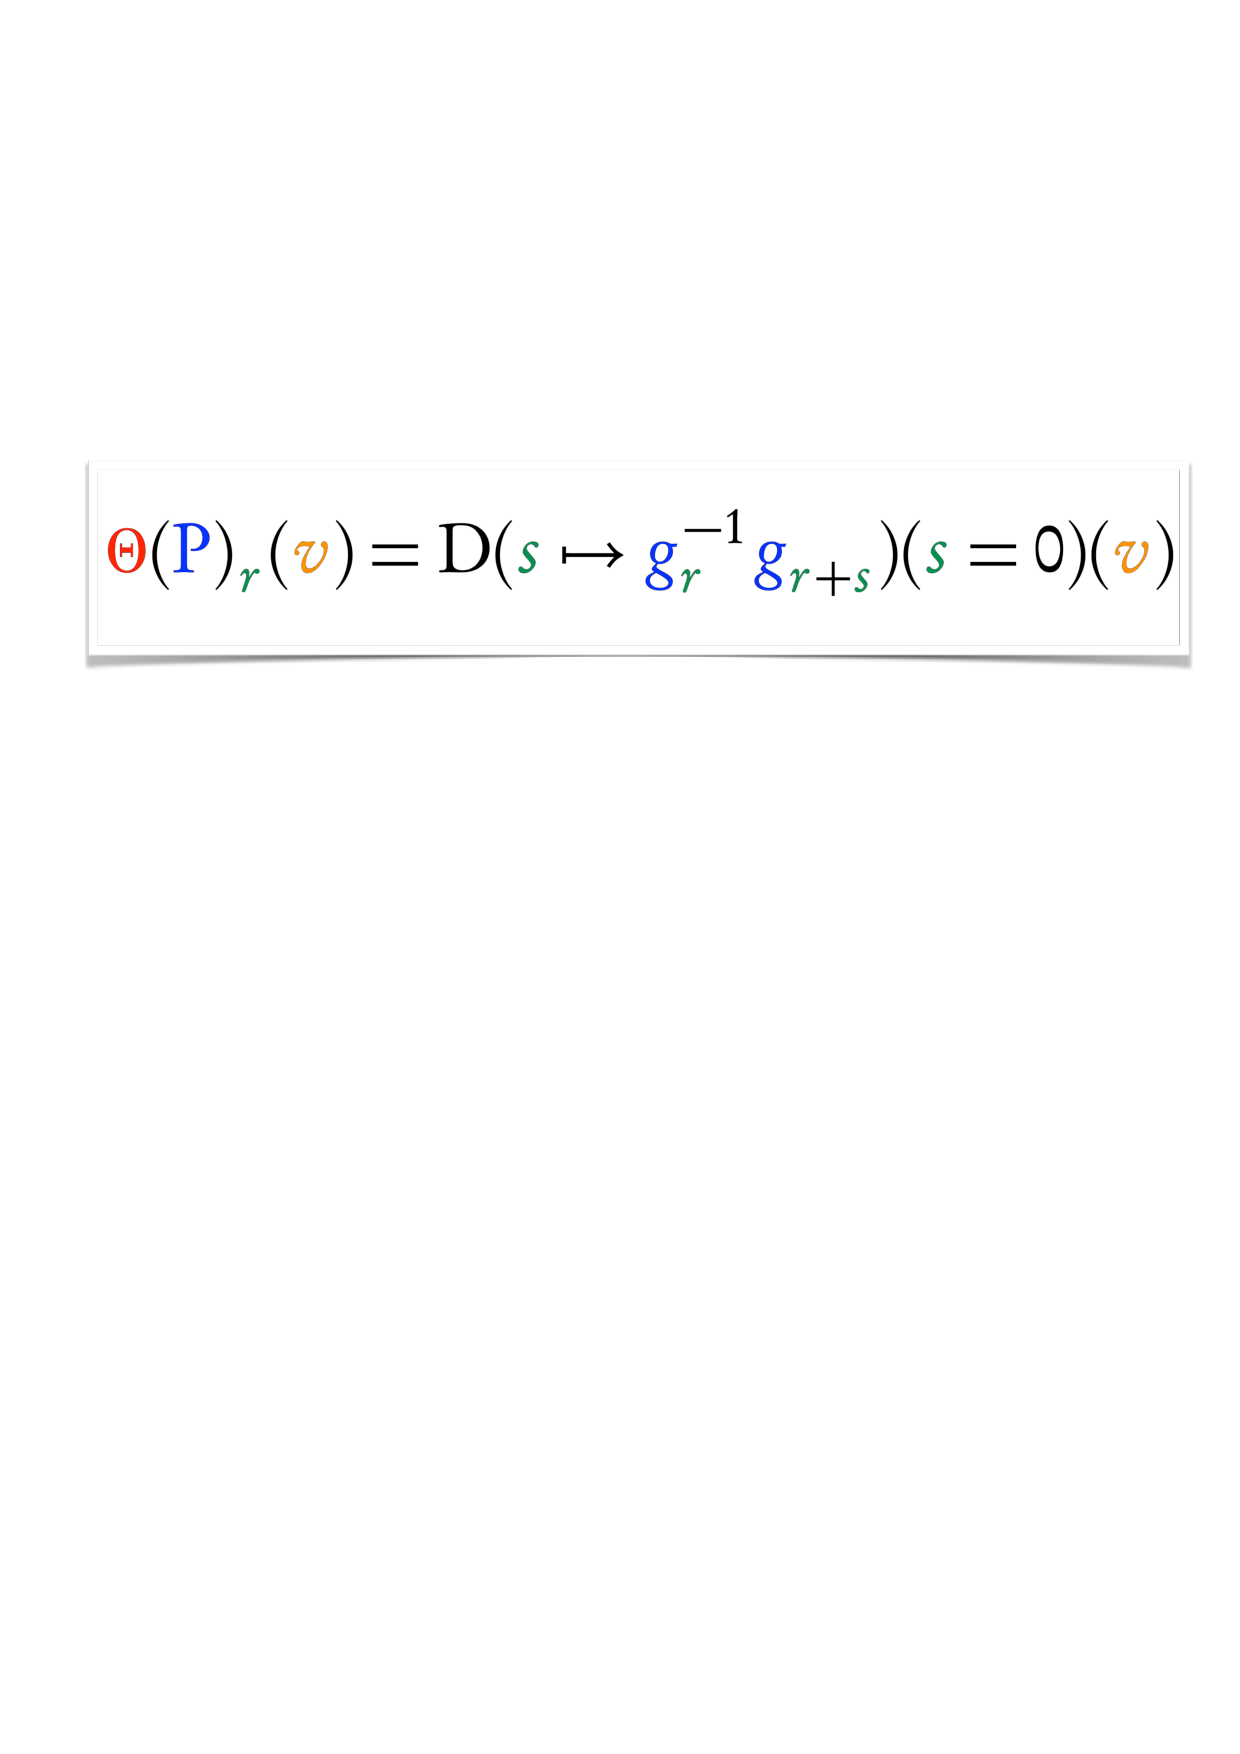
\includegraphics[width=\textwidth]{Figures/Maurer-Cartan.pdf}}
